\documentclass[10pt,a4paper]{article}
    \usepackage[hyperref]{acl2019}
    \usepackage{times}
    \usepackage{latexsym}
    \usepackage{graphicx}
    \usepackage{float}
    \usepackage{url}
    
    \aclfinalcopy % Uncomment this line for the final submission
    %\def\aclpaperid{***} %  Enter the acl Paper ID here
    
    %\setlength\titlebox{5cm}
    % You can expand the titlebox if you need extra space
    % to show all the authors. Please do not make the titlebox
    % smaller than 5cm (the original size); we will check this
    % in the camera-ready version and ask you to change it back.
    
    \newcommand\BibTeX{B\textsc{ib}\TeX}
    
    \title{Parallel Programming CSCI 4320 Project Report: \\
    City Traffic Discrete Event Simulation}
    \author{Alex Garten \\
      RPI \\
      \texttt{gartea@rpi.edu} \\\And
      Shoshana Malfatto \\
      RPI \\
      \texttt{malfas@rpi.edu} \\}
    
    \date{}
    
    \begin{document}
    \maketitle
    \begin{abstract}
        We implemented a parallel discrete event simulator for traffic patterns at intersections using C and MPI.
    \end{abstract}
    
    \section{Introduction}
    
    Our goal was to implement a parallel discrete event simulator which models vehicle traffic patterns to reveal which traffic rules result in the shortest trips between a location A and location B, in a large grid modeled after a city. Though implementations of traffic pattern DES already exist, we will use this as an opportunity to learn how to create a DES, since they have many applications.
    
    \section{Background}
    Our knowledge of parallel discrete event simulators (PDES) comes originally from the course lecture. Parallel DES help represent large-scale systems that are hard to understand, and which may require long run times if represented in real-time. A parallel DES should significantly reduce the run time. For instance, a simulation of air traffic could take a few minutes instead of a several years by looking at only specific events that are deemed important, and looking at them in parallel when possible. This could be applied to many other topics like communication networks or biology. An old article \cite{Fujimoto:1990:PDE:84537.84545} that contains some of the information from class provided a good overview of what discrete event simulators can consist of.
    
    When designed a PDES it is important to consider what type of synchronization algorithm to use. There are fundamentally two different types of synchronization algorithms: conservative algorithms and optimistic algorithms \cite{Fujimoto:1993:PDD:256563.256596}. Conservative algorithms guarantee that each event is safe to process. For simplicities sake this is the type of algorithm we attempted. Optimistic algorithms do not guarantee that each event is safe to process, but when a mistake does occur it roles back to the necessary timestamp and ensures that the mistake is not repeated. Given more time we would've likely used this type of algorithm. A good comparison is given in \cite{Carothers:2010}
    
    In class we talked about Rensselaer’s Optimistic Simulation System (ROSS) \cite{Barnes:2013:WSE:2486092.2486134} which runs Time Warp, a protocol that increases parallelism through rollback and anti-message mechanisms. This protocol scales very well in performance tests on RPI's Blue Gene/Q. We could have chosen to use ROSS to build our implementation, or looked into OMNeT++ \cite{Varga:2008:OOS:1416222.1416290}, which a popular open-source discrete event simulation environment, but we decided to create our simulator from scratch. 
    
    A significant amount of work has already been done in modeling traffic. There a variety of different methods used to model traffic but they models are usually macroscopic, mesoscopic, microspic. Macroscopic models maintain traffic as a indivisible flow while microspic models describe individual drivers. Mesoscopic lies somewhere in the middle. Macroscopic models are used mostly in plannins as in \cite{Salem:1994}. Various versions of mesoscopic models have been created, CONTRAM \cite{CONTRAM:1989} for example represents traffic as a network of nodes and links with the vehicles in those links grouped as packets. DYNAMIT \cite{Ben-AKiva:2001} used individual vehicles moving along segments according to queuing models and speed-density relationships. DYNASMART \cite{Jayakrishnan:1994} used a more detailed representation of intersections rather than queuing models but kept the speed-density relationships to help better model delays. FASTLANE \cite{Gawron:1998} replaces the speed-density relationships with a stochastic queue. This helps better represent interactions between different street elements. Lane changing is included in this. More recently hybrid models \cite{Burghout:2005} have started to appear. CTRRIT \cite{Burghout:2006} developed a hybrid mesoscopic-micrsopic model to better capture the larger effects on local traffic phenomenon. Their traffic network representation is a graph of nodes and links. Links are unidirectional and with no lanes represented are the only source of friction.
    
    Until recently their has not been enough research into traffic simulation in a High Performance environment. With an ever increasing complexity in transportation systems it is becoming increasingly necessary for stakeholders to design accurate models to make good transportation policy. Complex emerging technologies such as automation and deeper connectivity will require ever more complex control methods. As it is faster, more efficient and cheaper to model these control methods, it is increasingly important that traffic simulations be fast. MIBILITI \cite{MOBILIT:2018} has attempted to meet this need by building a scalable transportation simulation. MIBILITI is an Agent based simulator with road networks as agents and vehicles as events. They use an optimistic model with design concepts to minimize the amount of rolled back events. Interestingly they used GASNet and more of a master/slave aproach instead of MPI. The simulator is built on top of the Devastator parallel event simulator. Their simulator scaled aproximately linearly with a 2x increase in core count creating a 2x speedup. Other agent based traffic frameworks exist such as POLARIS \cite{SOKOLOV2012854} and MATSIM \cite{Waraich2015} though these are more conservative that MOBILITI.
    
    Other approaches have been tried. Dispite SIMD architecture not known to be good for network traffic simulation due to random memory access, Strippen \cite{Strippgen:2009}had a decent amount of success at optimizing the simulation. The key benefit of this approach is it allowed for a significant amount of extra computation for a very low prices.
    \section{Implementation}
    
    Our work attempts to bring together traffic models with High Performance Computing (HPC). Although much work has been done in modeling traffic and much work has been done in HPC there remains a gap in bridging the two. We started with an implementation with a more complex grid, but started having memory errors close to the deadline which we would have struggled to find in time for submission, so we went with a simpler grid for our second implementation. However, that also failed due to a deadlock issue. With little time left we changed and went for a 3rd much simpler implimentation. we will go over the initial two implementations since those have a significant amount of relevant learning experiance.
    
    \subsection{Implementation 1}
    
    We used a conservative approach to build our parallel DES, where cars can stop at a discrete number of locations, and at most one movement could occur within a tick. In our large city, which was a grid of streets going either north-south or east-west, cars only needed to know about the cars near them, so traffic could run somewhat independently in different regions. However, synchronization is required to accurately move cars across the borders of their region.
    
    For parallelization we used MPI, which we preferred to relying on threads after seeing the performance of both in Assignment 4/5. We used a side length for our grid of 32,768 blocks. For the full number of rows, this was multiplied by 2 so that even rows correspond to global coordinates of east-west streets, and odd rows correspond to global coordinates of north-south streets. The rows get divided up by the number of ranks, so that there would need to be communication with "ghost rows" like in homework 4/5.
    
    \begin{figure}
        \centering
        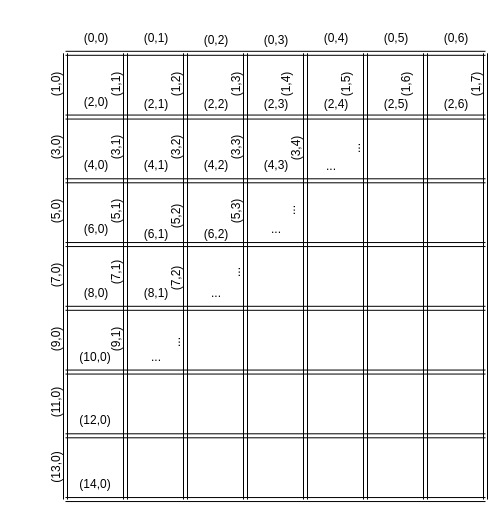
\includegraphics[scale=0.4]{parallel.jpg}
        \caption{Original street design, with  streets (where you consider a street as just one block). The global index is displayed for some of the streets. Even row indices correspond to horizontal streets, and odd row indices correspond to vertical streets.}
        \label{fig:my_label}
    \end{figure}
    
    Each street was a C struct that contained an array for the lane going in one direction (east or south) and the lane going in the opposite direction (west or north). Each lane could hold 4 cars at one time. This resembled a queue, which is a commonly seen data structure in discrete event simulators.
    
    There are intersection structs for each place where four streets should meet. This made moving cars cleaner for the programmer to implement and read.
    
    \begin{figure}
        \centering
        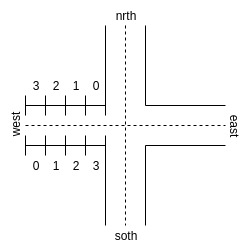
\includegraphics[scale=0.6]{parallel2.jpg}
        \caption{An intersection, including street indices from initial implementation (when each lane on a block had four locations). There can be at most 4 cars going through an intersection at a time.}
        \label{fig:my_label}
    \end{figure}
    
    The beginning of the simulation started with cars being randomly generated at locations on the grid, with random destinations. These locations are represented by a row index, a column index, and a street index which corresponds the eastern or southern direction. This was a very microspic model. 
    
    At each step in time, or 'tick', ghost rows were sent between ranks. This required sending arrays of car objects, which are not an MPI\_Datatype.
    
    Then intersections were updated according to the specified rules. Cars tried to turn in a direction that would get them closer to their destination on the global grid, but they must follow the rules of the road and not crash into other cars. For instance, if the car at the northern side of the intersection goes straight south, the car on the eastern side of the intersection can't go any direction but right within that tick of time. Then the streets would be updated by moving cars along them. Each car was supposed to move at most one grid location per tick.
    
    Our program worked with only 1 rank, but when multiple ranks were used, the program would terminate unexpectedly. There were so many places that memory could be used incorrectly, and parallel programs are difficult to debug, so after some time spent trying to discover the bug, we changed plans to a different implementation of the city traffic problem.
    
    \subsection{Implementation 2}
    
    \begin{figure*}
        \centering
        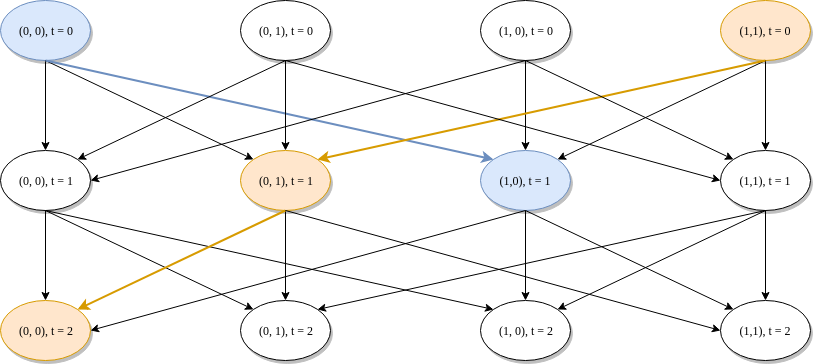
\includegraphics[scale=0.5]{imp2_diag.png}
        \caption{An model of the graph that implimentation 2 was supposed to solve. Here the blue car starting at 0,0 goal is to get to 1,0 and it does that at t=1. The orange car starts at 1,1 and its goal is to get to 0,0. It does that at t=2.}
        \label{fig:my_label}
    \end{figure*}
    
    
    After the faluire of our first try we attempted to simplify and refocus our simulation. We kept many of the same details from the initial implementation,but now there are only intersections and no streets. This reduced complexicity by eliminating much of the computation. This rather than being a microspic model was a macrospic model. We no longer had to manage street arrays or have complicated intersections traffic rules. The goal of the this implimentation was to refocus it on communication between MPI ranks. This refocus was also its downfall. 
    
    In our first implimentation although the traffic mechanics were complicated, the MPI exchange was actually quite simple. All data could be sent before each tick and the implimentation was parallel deterministic. However, due to some fundamentals the 2nd implimentation was not possible to be made parallel deterministic and required some difficult inter-rank communication. When updating an intersection, the intersection would have to check with its neighboring intersection to see if that intersection was already full in the current tick or in the previous tick. This was a trivial class within one mpi rank. This was not a trivial task between mpi ranks. To do this we developed a bit of an exchange protocol. The requesting rank would send a request with the data it wished to send. The answering rank would receive that data and if it was an eligible move, it would impliment the changes specified and send back a positive confirmation. If it was not an eligible move it would return a negative confirmation. With a positive confirmation the original rank would not continue any further as the move was completed by the other rank. With a negative confirmation the original rank would attempt to proceed knowing that the rank transitory move was not valid.
    The additional difficulty of this implimentation in order to keep it highly parallel was that the computation of own data needed to happen in parallel to the MPI communication. Although there
    were checks in place to make sure each rank answered all of its corresponding requests before moving,
    the system got deadlocked (some of the time with frequency scaling up with size of grid and number of ranks) with more than 2 ranks. We are not sure exactly what happened, but it is likely either some element of our protocol was incorrect or the checks got corrupted with an errounous send or receive
    deadlocking the system.
    This difficulty in protocol was magnified by the graph like nature of our problem. A visualization can be seen in figure 3. Each intersection at a point in time could be considered a node. The movement from a node to another at each tick could be considered an edge. To solve this graph the goal would be to find a non-overlapping path from each starting node to each ending node (technically a set of ending nodes as the time stamp of the node does not matter). The difficulty in solving graph based problems in parallel is well documented due to their incosistant and irregular nature. We definetly encountered this problem in this implimentation as receives had to be posted that never got sent to (and had to be resolved later which is likely where our deadlock issue was).
    Given more time it is likely we could've perfected this implimentation either through debugging or the adding of additional inefficiencies to ensure everything worked. 
    
    
    \subsection{Final Implementation}
    A visualization of the protocol can be seen in figure 4.
    
    \begin{figure*}
        \centering
        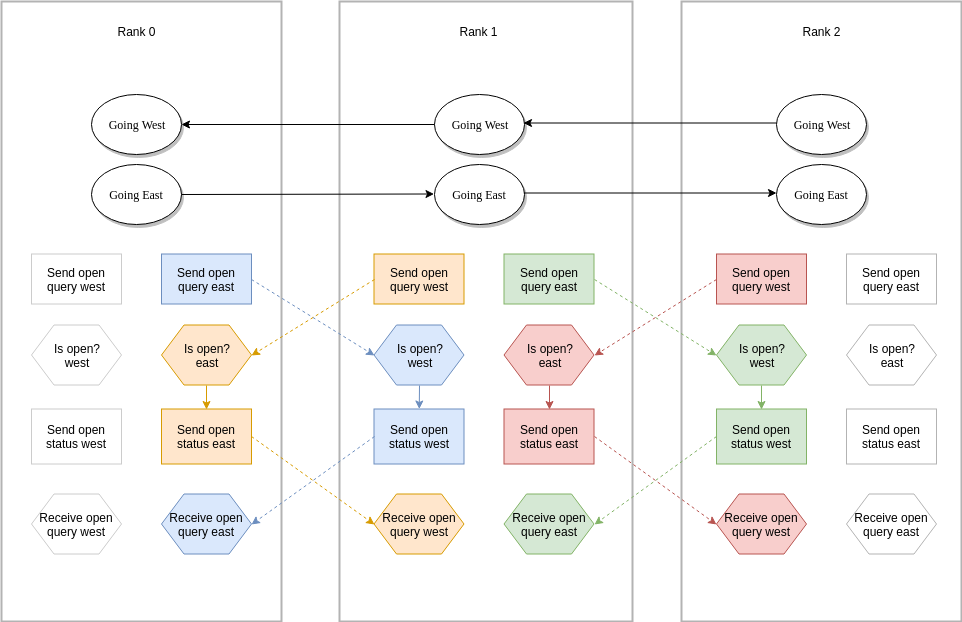
\includegraphics[scale=0.4]{imp3_diag.png}
        \caption{A model of the interprocess protocol for the 3rd implimentation. It does that at t=2.}
        \label{fig:my_label}
    \end{figure*}
    
    \section{Performance Results}
    
    \begin{figure}[H]
        \centering
        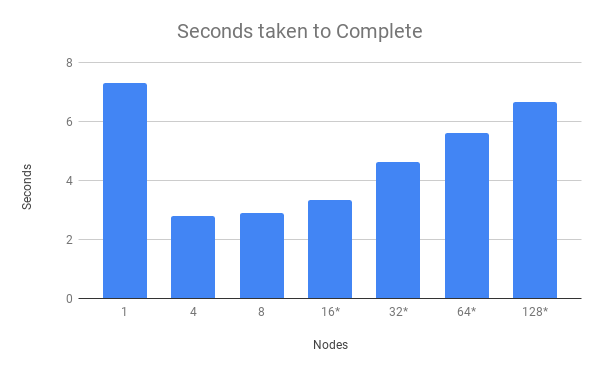
\includegraphics[scale=0.3]{seconds.png}
        \caption{The time of computation taken for additional nodes. * denotes extrapolated data}
        \label{fig:my_label}
    \end{figure}
    
    \begin{figure}[H]
        \centering
        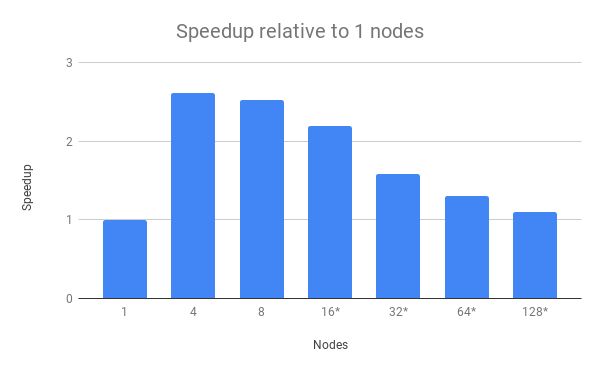
\includegraphics[scale=0.3]{speedup.png}
        \caption{The speedup over 1 node (64 ranks). * denotes extrapolated data}
        \label{fig:my_label}
    \end{figure}
    
    
    \section{Analysis of Performance}
    
    As you can see in our performance results our implimentation did not strong scale
    particularly well. Like all parallel implimentations, our implimentation is a race between inter-rank communicaiton and parallel computation. If there is too much inter rank communication then the amount of idle time created by the communication outweighs the reduced computation time by increased parallelism. With a highway of size 32K, we saw a maximun speedup at 4 nodes. Any additional nodes only slows down our implimentation.
    
    \section{Conclusion}
    
    \section{Team Organization}
    
    In our first version, Alex wrote all of the MPI code and the initial architecture, and Shoshana was working on updating intersections and streets according to traffic rules. For the second version, Alex wrote most of code and for the third version Shoshana wrote most of the 3rd version. Both wrote the report. Both team members ran jobs on the Blue Gene and debugged.
    
    \bibliographystyle{acl2019}
    \bibliography{acl_natbib}
    
    
    \end{document}
    